\documentclass{article}
\usepackage{listings}
\usepackage{color}
\usepackage{amsmath}
\usepackage{mathtools}
\usepackage{amsfonts}
\usepackage{amssymb}
\usepackage{caption}
\usepackage{tabularx}
\usepackage[export]{adjustbox}
\usepackage{polski}
\usepackage{indentfirst}
\usepackage{graphicx}
\usepackage{pdfpages}
\usepackage{float}
\usepackage{gauss}

\DeclareCaptionType{equ}[][List of equations]
\captionsetup[equ]{labelformat=empty}

%script adding bars in matrix
\usepackage{etoolbox}
\makeatletter
\patchcmd\g@matrix
 {\vbox\bgroup}
 {\vbox\bgroup\normalbaselines}% restore the standard baselineskip
 {}{}
\makeatother

\newcommand{\BAR}{%
  \hspace{-\arraycolsep}%
  \strut\vrule % the `\vrule` is as high and deep as a strut
  \hspace{-\arraycolsep}%
}
\definecolor{dkgreen}{rgb}{0,0.6,0}
\definecolor{gray}{rgb}{0.5,0.5,0.5}
\definecolor{mauve}{rgb}{0.58,0,0.82}

\lstset{frame=tb,
  language=Python,
  aboveskip=3mm,
  belowskip=3mm,
  showstringspaces=false,
  columns=flexible,
  basicstyle={\small\ttfamily},
  numbers=none,
  numberstyle=\tiny\color{gray},
  keywordstyle=\color{blue},
  commentstyle=\color{dkgreen},
  stringstyle=\color{mauve},
  breaklines=true,
  breakatwhitespace=true,
  tabsize=3,
  extendedchars=\true,
  inputencoding=utf8x
}

\lstset{literate={ą}{{\k{a}}}1 {ł}{{\l{}}}1 {ń}{{\'n}}1 {ę}{{\k{e}}}1 {ś}{{\'s}}1 {ż}{{\.z}}1 {ó}{{\'o}}1 {ź}{{\'z}}1 {Ą}{{\k{A}}}1 {Ł}{{\L{}}}1 {Ń}{{\'N}}1 {Ę}{{\k{E}}}1 {Ś}{{\'S}}1 {Ż}{{\.Z}}1 {Ó}{{\'O}}1 {Ź}{{\'Z}}1 }

\begin{document}
\title{Sprawozdanie - Metody numeryczne i optymailzacja}
\author{Jakub Andryszczak 259519,\\ Jakub Żak 244255,\\ Maciej Cierpisz 249163}
\date{}
\maketitle

\newpage
\tableofcontents
%Tutaj zaczyna się wstęp

\newpage
\section{Zadanie nr. 1}

\section{Zadanie nr. 2}
Sprawdź warunki optymalizacji pierwszego i drugiego rzędu dla funkcji kwadratowych:
\begin{equation}
  a) f(x) = 2x^2_1 - x_1x_2 + \frac{1}{2}x^2_2 - 3x_1 + 3.5,
\end{equation}
\begin{equation}
  a) f(x) = -\frac{3}{2}x^2_1+x_1x_2-\frac{1}{2}x^2_2 +2x_1 - 1
\end{equation}
\begin{equation}
  a) f(x) = x^2_1 + 8x_1x_2 + \frac{1}{2} x^2_2 - 10x_1 - 9x_2 + \frac{9}{2}
\end{equation}
Narysuj ich wykresy konturowe. Czy te funkcje są wypukłe? Jaki rodzaju stacjonarność
występuje w tych funkcjach?\newline

a) do sprawdzenia optymalizacji pierwszego rzędu dla funkcji kwadratowej należy wyliczyć gradient tej funkcji.
\begin{equation}
  \nabla f(x) =
  \begin{gmatrix}[b]
    4x_1-x_2-3\\-x_1+x_2
  \end{gmatrix}
\end{equation}
Następnie wyliczony wartoci wektora x. Do tego należy $\nabla f(x^*)=0$.
\begin{equation}
    \begin{cases}
      4x_1-x_2-3=0\\
      -x_1+x_2=0
    \end{cases}
\end{equation}
Po przeliczeniu wyszło, że wektor dla tej funkcji jest równy:
\begin{equation}
  x=\begin{gmatrix}[b]
    1\\1
  \end{gmatrix}
\end{equation}
Do policzenia drugiego rzędu należy wyliczyć hesian tej funkcji. Pozwoli to nam wyznaczyć czy funkcja jest wypukła.
\begin{equation}
  H= 
  \begin{gmatrix}[b]
    4&-1\\-1&1
  \end{gmatrix}
\end{equation}
kolejno należy wyliczyć wyznacznik dla $det(H-I\lambda)$.
\begin{equation}
  det(H-I\lambda) = (4-\lambda)(1-\lambda)-1
\end{equation}
\begin{equation}
  \lambda_1 = \frac{5-\sqrt[]{13}}{2}
\end{equation}
\begin{equation}
  \lambda_1 = \frac{5+\sqrt[]{13}}{2}
\end{equation}
Obie wartości są dodatnie, a zatem funkcja należy do wypukłych. Wykres Wygenerowany w Geogebrze wygląda następująco.
\begin{figure}[h]
  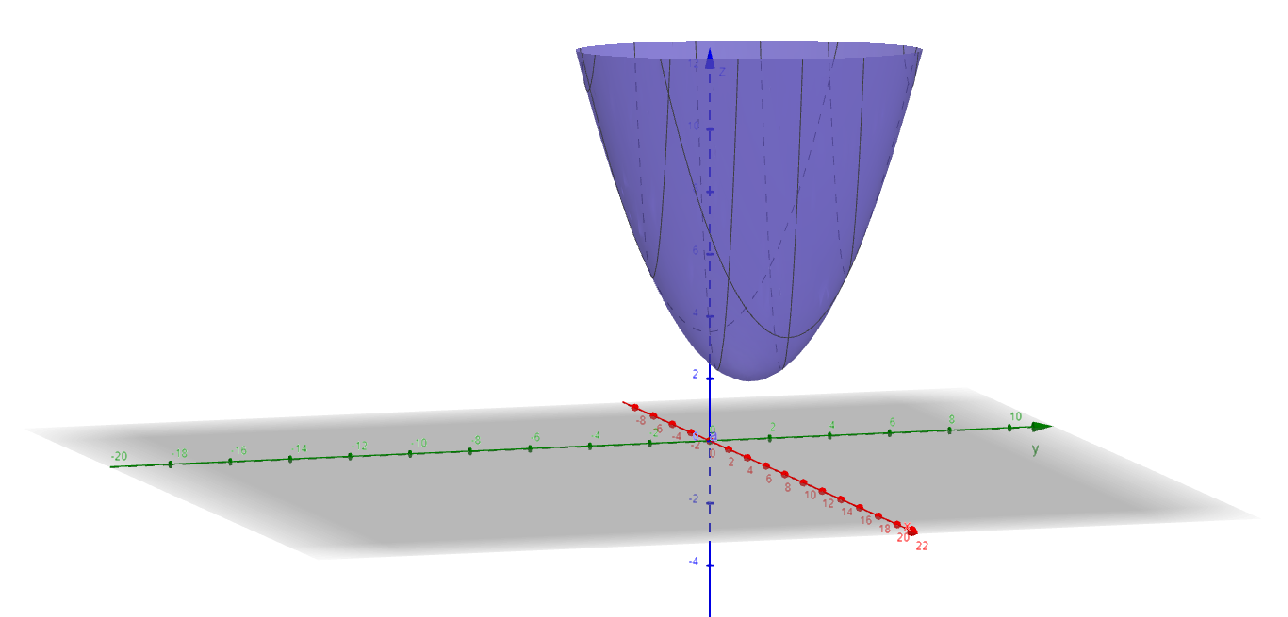
\includegraphics[scale=0.4]{Zadanie2a-wykres.png}
  \title{Rys 2.1 Wykres 3d funkcji podpunktu a)}
  \centering
\end{figure}

Dla podpunktu b) i c) wykonano podobne obliczenia dlatego pominięto rozpisywanie wszystkiego krok po kroku.
b)
\begin{equation}
  \nabla f(x)=
  \begin{gmatrix}[b]
    -3x_1+x_2+2\\ x_1-x_2
  \end{gmatrix}
\end{equation}
\begin{equation}
  x=\begin{gmatrix}[b]
    1\\1
  \end{gmatrix}
\end{equation}
\begin{equation}
  H=\begin{gmatrix}[b]
    -3&1\\1&-1
  \end{gmatrix}
\end{equation}
\begin{equation}
  det(H-I\lambda)=\lambda^2+4\lambda+2
\end{equation}
\begin{equation}
  \lambda_1=-2+\sqrt[]{2}
\end{equation}
\begin{equation}
  \lambda_2=-2-\sqrt[]{2}
\end{equation}
W tym przypadku obie lambdy są ujemne, a zatem funkcja jest funkcją wklęsłą.
\begin{figure}[h]
  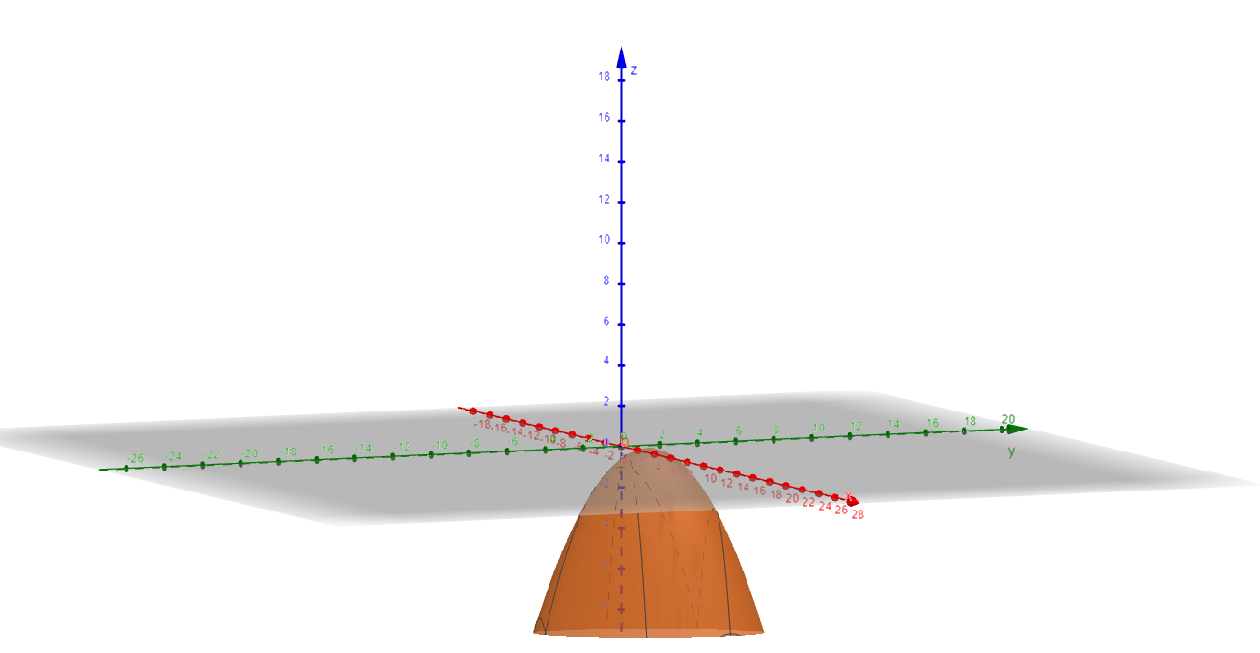
\includegraphics[scale=0.4]{Zadanie2b-wykres.png}
  \title{Rys 2.2 Wykres 3d funkcji podpunktu b)}
  \centering
\end{figure}
\newpage
c)
\begin{equation}
  \nabla f(x) =\begin{gmatrix}[b]
    2x_1+8x_2-10\\8x_1+x_2-9
  \end{gmatrix}
\end{equation}
\begin{equation}
  x=\begin{gmatrix}[b]
    1\\1
  \end{gmatrix}
\end{equation}
\begin{equation}
  H=\begin{gmatrix}[b]
    2&8\\8&1
  \end{gmatrix}
\end{equation}
\begin{equation}
  det(H-I\lambda)=\lambda^2-3\lambda-62
\end{equation}
\begin{equation}
  \lambda_1=\frac{3-\sqrt[]{257}}{2}
\end{equation}
\begin{equation}
  \lambda_2=\frac{3+\sqrt[]{257}}{2}
\end{equation}
W tym wypadku rozwiązania wychodzą jedna ujemna i jedna nieujemna. Wskazuje to na to, że funkcja nie ma globalnego minimum ani maksimum. Kształtem przypomina siodło, stąd nazwa "punkt siodłowy"
\begin{figure}[h]
  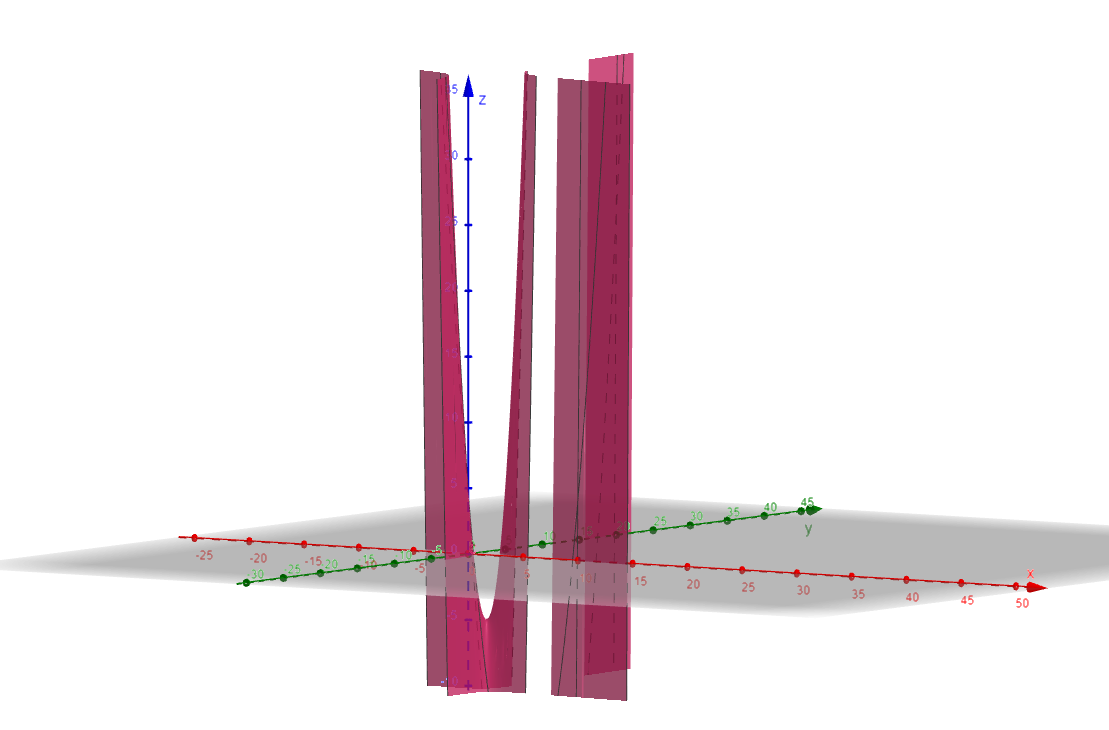
\includegraphics[scale=0.4]{Zadanie2c-wykres.png}
  \title{Rys 2.3 Wykres 3d funkcji podpunktu c)}
  \centering
\end{figure}
\newpage
\section{Zadanie nr. 3}
Dla funkcji kwadratowej:\\
\begin{equation}
  f(x) =   (x^T)Gx, gdzie \: G = \begin{gmatrix}[b]
    \alpha&1&1\\
    3&2&1\\
    2&2&3
  \end{gmatrix}
\end{equation}

Określić parametr, dla którego ta funkcja jest ściśle wypukła.\\
\newline

Funkcja f(x) jest ściśle wypukła, jeżeli wszystkie minory główne macierzy mają
dodatnie wyznaczniki. A zatem, jeżeli:

\begin{equation}
  det[\alpha] >  0\\
\end{equation}

\begin{equation}
  det
  \begin{gmatrix}[b]
    \alpha&1\\
    3&2
  \end{gmatrix}
  > 0
\end{equation}

\begin{equation}
  det
  \begin{gmatrix}[b]
    \alpha&1&1\\
    3&2&1\\
    2&2&3
  \end{gmatrix}
  > 0
\end{equation}

\begin{equation}
  \begin{cases}
    \alpha > 0\\
    \alpha \cdot 2 - 1 \cdot 3 > 0\\
    \alpha \cdot 2 \cdot 3 + 3 \cdot 2 \cdot 1 + 2 \cdot 1 \cdot 1 - 1 \cdot 2 \cdot 2 - 
    1 \cdot 2 \cdot \alpha - 3 \cdot 1 \cdot 3 >0
  \end{cases}
\end{equation}

\begin{equation}
  \begin{cases}
    \alpha > 0\\
    2\alpha > 3\\
    4\alpha >5
  \end{cases}
\end{equation}

\begin{equation}
  \begin{cases}
    \alpha > 0\\
    \alpha > \frac{3}{2}\\
    \alpha >\frac{5}{2}
  \end{cases}
\end{equation}


Liczba, która spełnia wszystkie trzy warunki to $\frac{2}{3}$, a zatem funkcja będzie ściśle
wypukła, jeżeli wartość parametru $\alpha$ będzie większa niż $\frac{3}{2}$.

\section{Zadanie nr. 4}

\section{Zadanie nr. 5}

\section{Zadanie nr. 6}

Zadana jest funkcja Rosenbrocka: $f(x)=100(x_2-x_1^2)^2+(1-x)^2$, narysuj
jej izolinie, a następnie znajdź jej lokalne minimum przy pomocy metod Fletchera-Reevesa
i Polaka-Ribiere'a, zaczynając od punktu początkowego: $x_0=\begin{gmatrix}[b]
  -1.2 & 1
\end{gmatrix}^T$.\\

Na potrzeby tego zdania wykorzystano algorytmy Fletchera-Reevesa
oraz Polaka-Ribiere’a. Listing kodu przedstawiono poniżej.

\begin{lstlisting}
  import numpy as np
  import matplotlib.pyplot as plt
  from matplotlib.colors import LogNorm
  from scipy.optimize import minimize
  
  # Definicja funkcji Rosenbrocka
  def rosenbrock(x):
      return 100*(x[1] - x[0]**2)**2 + (1 - x[0])**2
  
  # Wygenerowanie siatki punktow wokoł obszaru, w którym chcemy narysowac izolinie
  x = np.linspace(-2, 2, 100)
  y = np.linspace(-1, 3, 100)
  X, Y = np.meshgrid(x, y)
  Z = rosenbrock([X, Y])
  
  # Narysowanie izolinii funkcji Rosenbrocka
  plt.figure()
  plt.contour(X, Y, Z, levels=np.logspace(0, 3, 20), norm=LogNorm(), cmap=plt.cm.jet)
  plt.colorbar(label='Wartosc funkcji Rosenbrocka')
  plt.xlabel('x1')
  plt.ylabel('x2')
  plt.title('Izolinie funkcji Rosenbrocka')
  plt.show()
  
  # Definicja punktu początkowego
  x0 = np.array([-1, 2])
  
  # Implementacja algorytmu optymalizacji z metodą Fletchera-Reevesa
  result_fr = minimize(rosenbrock, x0, method='CG', jac=None, tol=1e-6)
  print("Minimum (Fletchera-Reevesa):", result_fr.x)
  
  # Implementacja algorytmu optymalizacji z metodą Polaka-Ribiere'a
  result_pr = minimize(rosenbrock, x0, method='BFGS', jac=None, tol=1e-6)
  print("Minimum (Polaka-Ribiere'a):", result_pr.x)
\end{lstlisting}  

W przypadku metody Fletchera-Reevesa, wykorzystano method='CG', gdzie CG oznacza metodę gradientową, 
która wykorzystuje algorytm sprzężonych gradientów (CG), który jest implementacją metody Fletchera-Reevesa.

Natomiast w przypadku metody Polaka-Ribiere'a, wykorzystano method='BFGS', gdzie BFGS oznacza metodę quasi-Newtona, 
która wykorzystuje algorytm Quasi-Newtona, w tym przypadku metoda Polaka-Ribiere'a.

Poniżej przedstawiono wynik działania kodu

\begin{lstlisting}
Minimum (Fletchera-Reevesa): [0.99999552 0.99999102]
Liczba iteracji (Fletchera-Reevesa): 34

Minimum (Polaka-Ribiere'a): [0.99999552 0.99999104]
Liczba iteracji (Polaka-Ribiere'a): 37
\end{lstlisting}

\begin{figure}[h]
   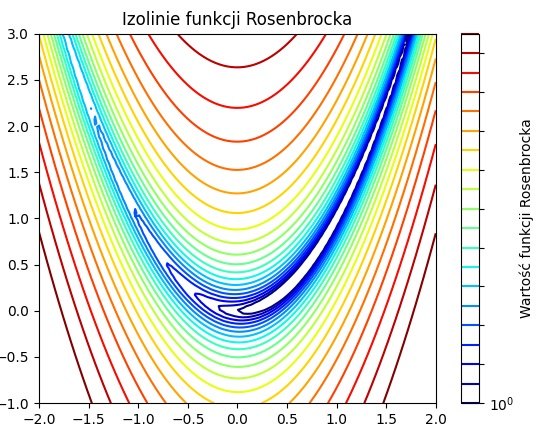
\includegraphics[scale=0.7]{zad6.jpg}
   \centering
\end{figure}

\section{Zadanie nr. 7}

Korzystając z algorytmów takich jak quasi-Newton oraz CG, rozwiązać układ
równań liniowych: Ax = b, gdzie $A=[a_{ij}] \epsilon \mathfrak{R}^{NxN}, a_{ij} = \frac{1}{i+j-1}$ jest macierzą
Hilberta, $b = [1, ..., 1] \epsilon \mathfrak{R}^N$. Rozpocząć iterację od $x_0 = 0$. Jeśli nie jest to
określone przez algorytm, do pomiaru błędu residualnego należy użyć odległości
euklidesowej. Wypróbować wymiary $N = 5, 8, 12, 20$ podać liczbę iteracji
potrzebnych do zmniejszenia błędu residualnego poniżej $10^{-6}$.\\

Na potrzeby tego zdania wykorzystano kod przedstawiony na listingu poniżej.

\begin{lstlisting}
  import numpy as np
  from scipy.optimize import minimize
  from scipy.sparse.linalg import cg
  
  def hilbert_matrix(n):
      """
      Funkcja tworząca macierz Hilberta o rozmiarze nxn.
      """
      return np.array([[1/(i + j - 1) for j in range(1, n+1)] for i in range(1, n+1)])
  
  def residual_error(x, A, b):
      """
      Oblicza blad residualny ||Ax - b||.
      """
      return np.linalg.norm(np.dot(A, x) - b)
  
  # Wymiary macierzy Hilberta
  N_values = [5, 8, 12, 20]
  
  for N in N_values:
      A = hilbert_matrix(N)
      b = np.ones(N)
      x0 = np.zeros(N)
      
      # Metoda quasi-Newtona (BFGS)
      result_bfgs = minimize(residual_error, x0, args=(A, b), method='BFGS', tol=1e-6)
      iterations_bfgs = result_bfgs.nit
      
      # Metoda gradientów sprzezonych (CG)
      x_cg, info_cg = cg(A, b, x0=x0, tol=1e-6)
      iterations_cg = 0 if isinstance(info_cg, int) else len(info_cg)
      residual_cg = np.linalg.norm(np.dot(A, x_cg) - b) if isinstance(info_cg, int) else info_cg
      
      print(f"Rozmiar macierzy: {N}")
      print(f"Liczba iteracji (BFGS): {iterations_bfgs}")
      print(f"Liczba iteracji (CG): {iterations_cg}")
      print(f"Residuum (CG): {residual_cg}")
  
\end{lstlisting}

Wyniki działania kodu przedstawiono poniżej.

\begin{figure}[h]
 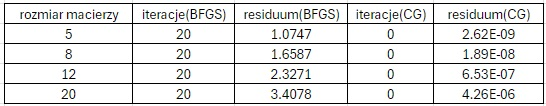
\includegraphics[scale=0.7]{zad7.jpg}
  \centering
\end{figure}

Metoda BFGS (quasi-Newton) zakończyła się dla każdego rozmiaru macierzy po 20 iteracjach.
Liczba iteracji dla metody CG (gradientów sprzężonych) wynosiła 0 dla każdego rozmiaru macierzy, co sugeruje, 
że metoda osiągnęła wymaganą dokładność w jednej iteracji.
Residuum dla metody CG było bardzo niskie dla każdego rozmiaru macierzy, 
co wskazuje na dobrą jakość rozwiązania.
Residuum dla metody BFGS było większe niż dla metody CG, co jest zrozumiałe, 
ponieważ metoda BFGS nie działa bezpośrednio na residuum.
\end{document}